
What is a satellite simulator and why it is needed?\\
Motivation of cloud simulator for ESA Cloud\_cci project:
Evaluation of the representation of clouds in ERA-Interim reanalysis data using CCI observations.\\
Summary of literature research, ERA-I and cloud simulators.\\
Text below must be summarized in own wording and shortened!\\


% Notizen aus Publikationen
% COSP, Bodas-Salcedo et al. (2011), BAMS
\cite{Bodas2011} Basic problem:\\
Models operate with spatial resolutions from a few kilometers to hundreds of kilometers.
Many atmospheric processes (e.g. turbulence, cloud formation, etc.) operate at smaller scales, 
which cannot be resolved by current global (regional?) model resolutions.
These processes are implemented via parameterizations (e.g. CER formula in ERA-I - explain in more detail),
which are based on semiempircal or statistical models that relate grid box mean variables
to subgrid processes. Thus, evaluation of parameterizations in models is essential to improve
weather forecasts or increasing our confidence in climate projections.\\
Satellite measurements are important for evaluating GCMs because they provide global observations.
But they measure photon counts (e.g. radiance, brightness temperature) and not directly the geophysical quanities
(e.g. cloud phase, number of cloud condensates, etc.).
Satellite retrievals utilize the measured intensity of radiation from a particular area and direction 
at a particular wavelength to infer by inverse modeling the cloud parameters.\\
Another difficulty is that cloud parameters defined in models do not necessarily match the satellite-based
cloud parameter definition. Then an inter-comparison between model and satellite derived products is not feasible.
Hence, cloud simulators are required to make them comparable and enabling the evaluation of the model or the retrieval.
Furthermore satellite retrievals measure the top of the cloud, while models are resolved vertically.
Moreover, satellite sensors have limitations (e.g. finite sensitivity, fixed viewing geometry, etc).
Retrievals have limitations due to assumptions and auxiliary datasets used, e.g. retrieval may be sensitive to
the first guess of the atmospheric state that is used in the inversion.\\
Nonetheless, satellite-based cloud properties can be compared with model outputs, 
results can be interpreted if using a cloud simulator and consequently,
model deficiencies can be identified.\\
Main drawback of simulator approach: interpreting results in terms of physical processes may sometimes be
problematic because the comparison variables are not trivially related to any single geophysical quantity.\\

\cite{Pincus2012}\\
Cloud properties observed by spaceborne instruments differ from the way clouds are represented in models.
All satellite retrievals relate reflectance measurements to physical properties using simple models of the atmosphere.
Cloud/Instrument simulator can bridge this gap, it is a diagnostic tool that map the model representation
to synthetic observations so that differences can be interpreted as model error.
Cloud simulator converts the model state into synthetic observations.
Goal is to put model predictions and observations on the same footing so that differences
between the two can be unambiguously interpreted as model error.
Simulator emulates satellite-based results using model output as input.
However, simulators may themselve be restricted by limited information or by internal assumptions 
(e.g., single vertically and horizontally uniform cloud layer, fully cloudy pixel, liquid or ice, etc.).
Like all models, instrument simulators are incomplete and thus, have limitations.
For instance, observational artifacts cannot be reproduced by simulators, e.g.
artifacts caused by partly cloudy satellite pixel or viewing and illumination geometry.\\
Instrument simulators cannot entirely close the gap between models and observations of clouds, however,
there are broad regimes in which they work well.
For instance, neglecting those clouds with a verly low optical thickness, can lead to a more robust model
evaluation. 
\cite{Pincus2012} state that the total cloud fraction is a very fragile measure to be used in model
evaluation. Cleary, it is an easy derived parameter due to binary decision about presence or absence of
a cloud. However, the total cloud fraction strongly depends on spatial scale at which it is measured.
At the kilometer scales at current sensors, different assumptions can have dramatic impacts on the climatology.
Hence, the authors suggest to apply empirical filters to the models before evaluation in order to make the
comparison more robust (e.g., neglect clouds with COT less than 1.3).\\
The fidelity of GCMs can be judged by comparing simulations of the present day with observations.
Clouds have strong and variable impacts on the Earth's radiation budget and
are beside aerosols still the largest uncertaininties in GCMs.\\
Synthesizing CCI observations of clouds from model states.
Instrument simulators use the internal description of clouds in a model along with the retrieval
characteristics of an algorithm aiming at the generation of statistics that is provided by an observational dataset.
In general simulators consist of three parts:
1) a treatment of subgrid-scale variability,
2) the simulation of pixel-scale retrievals, and
3) the calculation of statistics.
The first step is necessary to account for the different spatial scales in GCMs and spaceborne instruments.
Subcolumns can be considered being small samples, each of which is assumed to be homogeneous. 
The large ensemble of subcolumns reproduces then the input statistics and any internal inhomogeneity in each grid cell.
Cloud-resolving models do not require such a downscaling.
The second step leads to synthetic pixel-level retrievals.
The third step aggregates collections of retrievals to produce temporal averages and joint histograms.


Shortly describe the major steps, see Fig.~\ref{fig:sim_over} 
(input, downscaler, pseudo-retrieval, building diagnostics) 
of the cloud simulator, which are explained in detail in Section~\ref{sec:sim}\\

%\captionsetup[subfloat]{position=top}
\begin{figure}[!htp]
 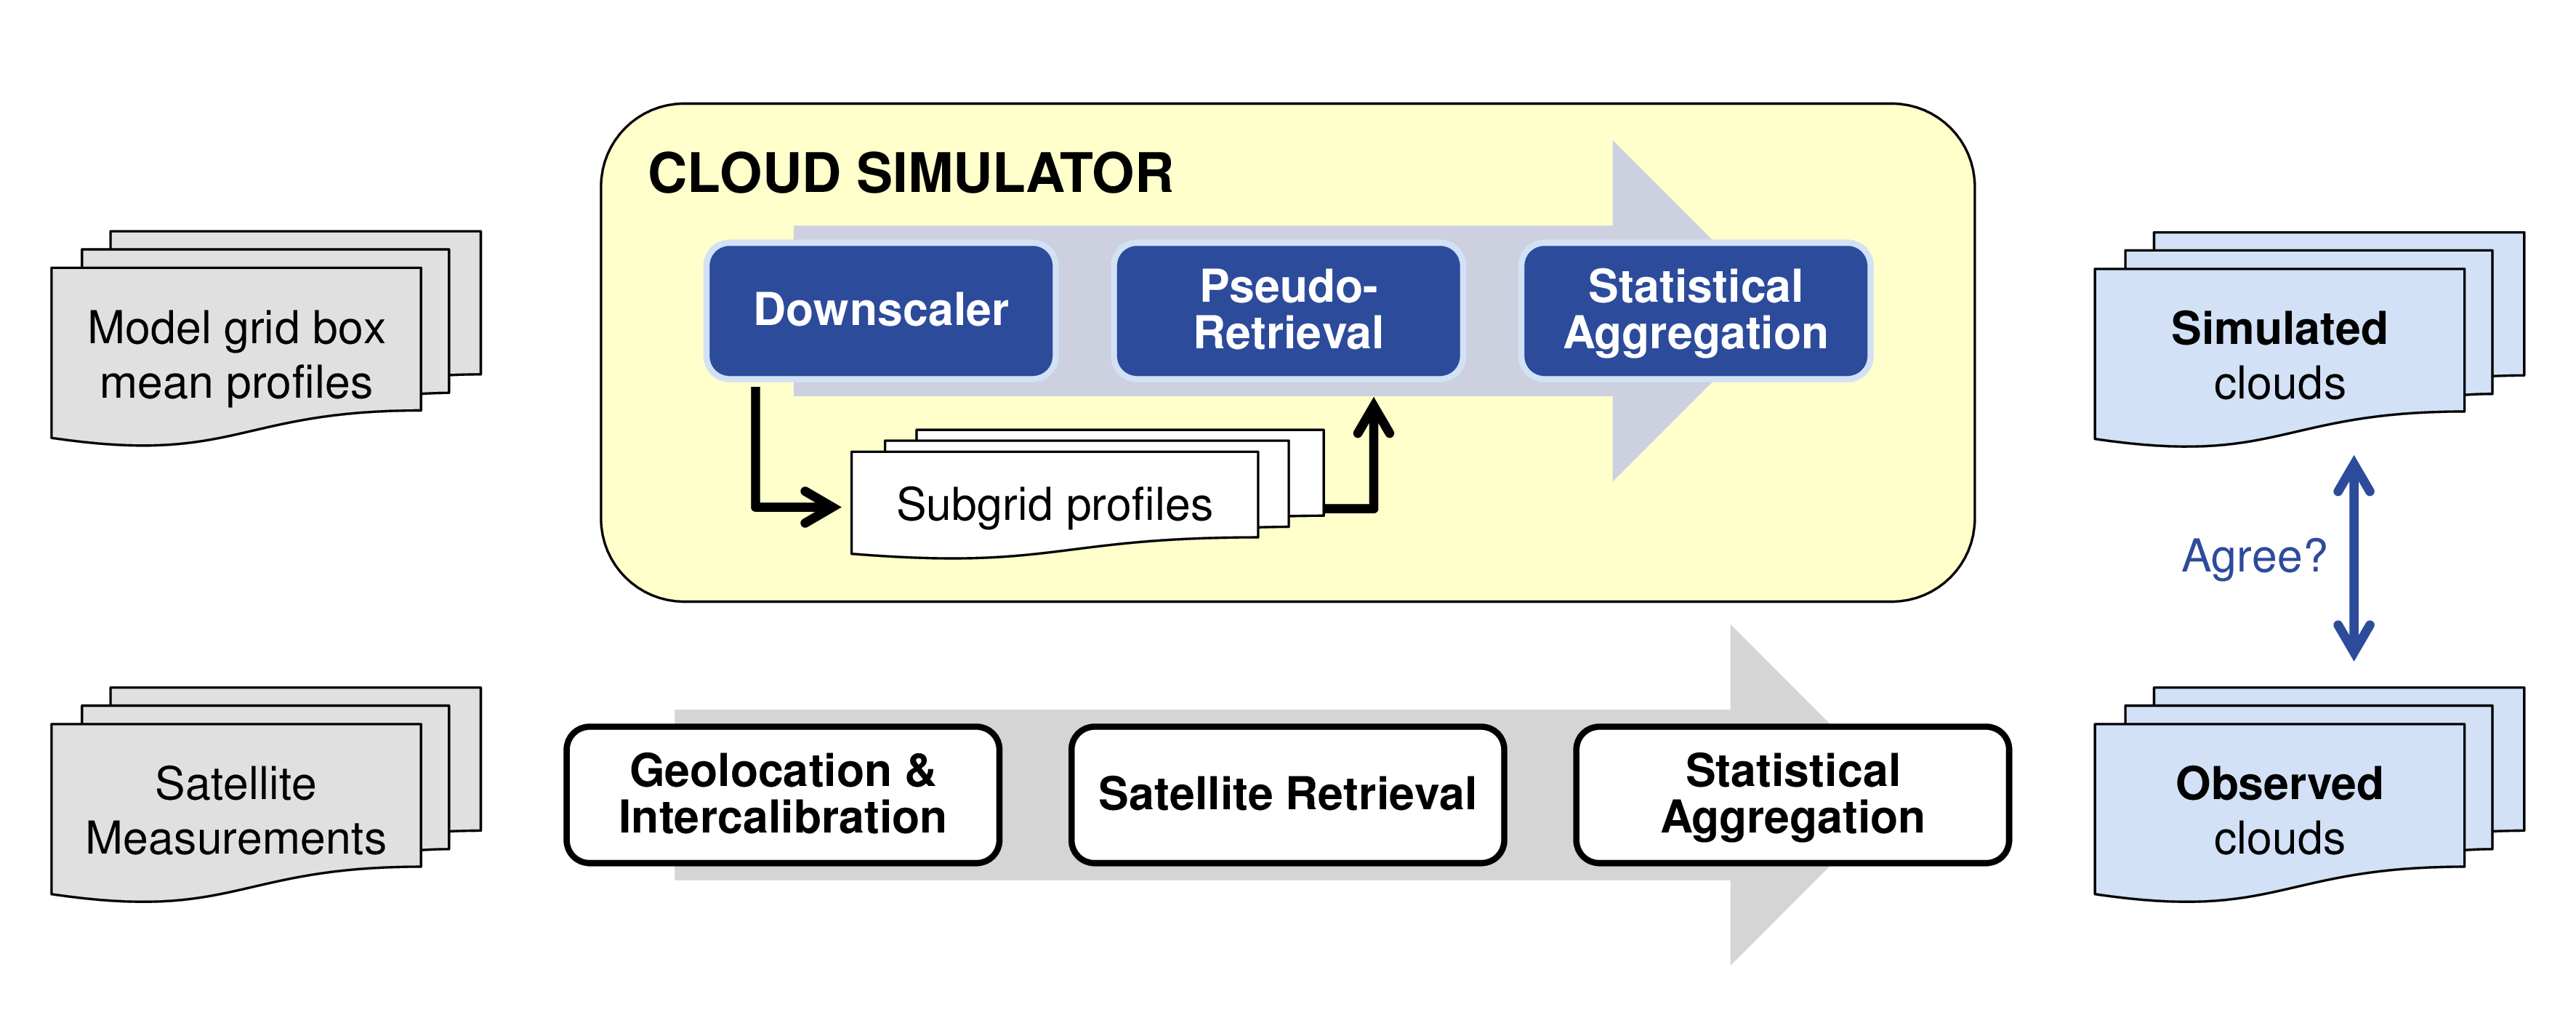
\includegraphics[width=\mapwidth]{./figures/simulator_overview.png}
  \caption[Concept of the cloud simulator.]
{Cloud simulator concept.}\label{fig:sim_over}
\end{figure}
